

\tikzset{every picture/.style={line width=0.75pt}} %set default line width to 0.75pt        

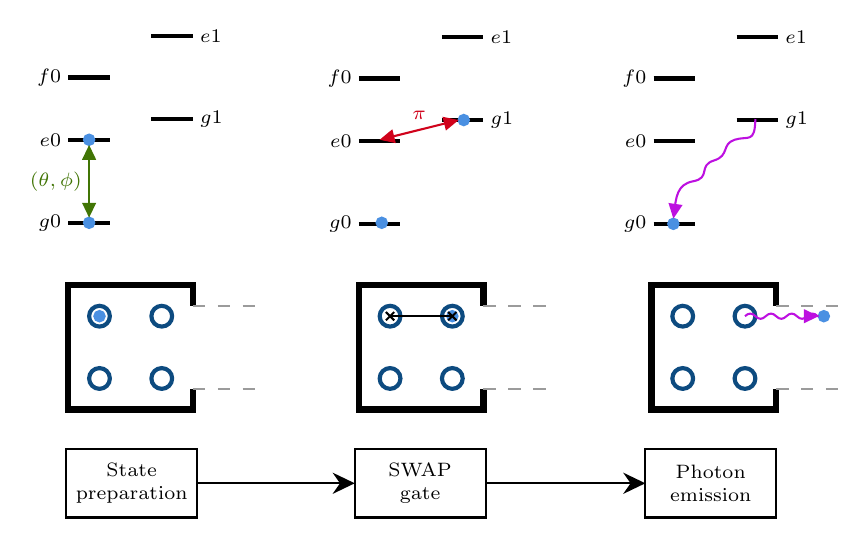
\begin{tikzpicture}[x=0.75pt,y=0.75pt,yscale=-1,xscale=1]
%uncomment if require: \path (0,472); %set diagram left start at 0, and has height of 472

%Straight Lines [id:da8931975658515314] 
\draw [line width=1.5]    (100,100) -- (120,100) ;
%Straight Lines [id:da6109179246921593] 
\draw [line width=1.5]    (140,80) -- (160,80) ;
%Straight Lines [id:da4740245259238267] 
\draw [line width=1.5]    (100,130) -- (120,130) ;
%Straight Lines [id:da8570593937301805] 
\draw [line width=1.5]    (100,170) -- (120,170) ;
%Straight Lines [id:da02915524605611408] 
\draw [line width=1.5]    (140,120) -- (160,120) ;
%Straight Lines [id:da16734412566121315] 
\draw [line width=1.5]    (240,100.5) -- (260,100.5) ;
%Straight Lines [id:da1741824563512493] 
\draw [line width=1.5]    (280,80.5) -- (300,80.5) ;
%Straight Lines [id:da23317779450869036] 
\draw [line width=1.5]    (240,130.5) -- (260,130.5) ;
%Straight Lines [id:da8493304549912968] 
\draw [line width=1.5]    (240,170.5) -- (260,170.5) ;
%Straight Lines [id:da9896717165480059] 
\draw [line width=1.5]    (280,120.5) -- (300,120.5) ;
%Straight Lines [id:da956624069338186] 
\draw [line width=1.5]    (382,100.5) -- (402,100.5) ;
%Straight Lines [id:da7887267818588047] 
\draw [line width=1.5]    (422,80.5) -- (442,80.5) ;
%Straight Lines [id:da03622865125847419] 
\draw [line width=1.5]    (382,130.5) -- (402,130.5) ;
%Straight Lines [id:da13614260982775128] 
\draw [line width=1.5]    (382,170.5) -- (402,170.5) ;
%Straight Lines [id:da1441695211618249] 
\draw [line width=1.5]    (422,120.5) -- (442,120.5) ;
%Shape: Circle [id:dp1759227411497647] 
\draw  [color={rgb, 255:red, 13; green, 75; blue, 128 }  ,draw opacity=1 ][line width=1.5]  (110,215) .. controls (110,212.24) and (112.24,210) .. (115,210) .. controls (117.76,210) and (120,212.24) .. (120,215) .. controls (120,217.76) and (117.76,220) .. (115,220) .. controls (112.24,220) and (110,217.76) .. (110,215) -- cycle ;
%Shape: Circle [id:dp4360171288549991] 
\draw  [color={rgb, 255:red, 13; green, 75; blue, 128 }  ,draw opacity=1 ][line width=1.5]  (110,245) .. controls (110,242.24) and (112.24,240) .. (115,240) .. controls (117.76,240) and (120,242.24) .. (120,245) .. controls (120,247.76) and (117.76,250) .. (115,250) .. controls (112.24,250) and (110,247.76) .. (110,245) -- cycle ;
%Shape: Circle [id:dp5194230164195629] 
\draw  [color={rgb, 255:red, 13; green, 75; blue, 128 }  ,draw opacity=1 ][line width=1.5]  (140,245) .. controls (140,242.24) and (142.24,240) .. (145,240) .. controls (147.76,240) and (150,242.24) .. (150,245) .. controls (150,247.76) and (147.76,250) .. (145,250) .. controls (142.24,250) and (140,247.76) .. (140,245) -- cycle ;
%Shape: Circle [id:dp7655825363179872] 
\draw  [color={rgb, 255:red, 13; green, 75; blue, 128 }  ,draw opacity=1 ][line width=1.5]  (140,215) .. controls (140,212.24) and (142.24,210) .. (145,210) .. controls (147.76,210) and (150,212.24) .. (150,215) .. controls (150,217.76) and (147.76,220) .. (145,220) .. controls (142.24,220) and (140,217.76) .. (140,215) -- cycle ;
%Shape: Square [id:dp010299027105199587] 
\draw  [line width=2.25]  (100,200) -- (160,200) -- (160,260) -- (100,260) -- cycle ;
%Straight Lines [id:da10238522924376559] 
\draw [color={rgb, 255:red, 255; green, 255; blue, 255 }  ,draw opacity=1 ][line width=3]    (160,210) -- (160,250) ;

%Shape: Circle [id:dp042388463572761714] 
\draw  [color={rgb, 255:red, 74; green, 144; blue, 226 }  ,draw opacity=1 ][fill={rgb, 255:red, 74; green, 144; blue, 226 }  ,fill opacity=1 ] (112.5,215) .. controls (112.5,213.62) and (113.62,212.5) .. (115,212.5) .. controls (116.38,212.5) and (117.5,213.62) .. (117.5,215) .. controls (117.5,216.38) and (116.38,217.5) .. (115,217.5) .. controls (113.62,217.5) and (112.5,216.38) .. (112.5,215) -- cycle ;
%Shape: Circle [id:dp10905807386965438] 
\draw  [color={rgb, 255:red, 13; green, 75; blue, 128 }  ,draw opacity=1 ][line width=1.5]  (250,215) .. controls (250,212.24) and (252.24,210) .. (255,210) .. controls (257.76,210) and (260,212.24) .. (260,215) .. controls (260,217.76) and (257.76,220) .. (255,220) .. controls (252.24,220) and (250,217.76) .. (250,215) -- cycle ;
%Shape: Circle [id:dp1368955719904016] 
\draw  [color={rgb, 255:red, 13; green, 75; blue, 128 }  ,draw opacity=1 ][line width=1.5]  (250,245) .. controls (250,242.24) and (252.24,240) .. (255,240) .. controls (257.76,240) and (260,242.24) .. (260,245) .. controls (260,247.76) and (257.76,250) .. (255,250) .. controls (252.24,250) and (250,247.76) .. (250,245) -- cycle ;
%Shape: Circle [id:dp9583422679674527] 
\draw  [color={rgb, 255:red, 13; green, 75; blue, 128 }  ,draw opacity=1 ][line width=1.5]  (280,245) .. controls (280,242.24) and (282.24,240) .. (285,240) .. controls (287.76,240) and (290,242.24) .. (290,245) .. controls (290,247.76) and (287.76,250) .. (285,250) .. controls (282.24,250) and (280,247.76) .. (280,245) -- cycle ;
%Shape: Circle [id:dp6563593124398152] 
\draw  [color={rgb, 255:red, 13; green, 75; blue, 128 }  ,draw opacity=1 ][line width=1.5]  (280,215) .. controls (280,212.24) and (282.24,210) .. (285,210) .. controls (287.76,210) and (290,212.24) .. (290,215) .. controls (290,217.76) and (287.76,220) .. (285,220) .. controls (282.24,220) and (280,217.76) .. (280,215) -- cycle ;
%Shape: Square [id:dp13654534966408327] 
\draw  [line width=2.25]  (240,200) -- (300,200) -- (300,260) -- (240,260) -- cycle ;
%Straight Lines [id:da4280868328748867] 
\draw [color={rgb, 255:red, 255; green, 255; blue, 255 }  ,draw opacity=1 ][line width=3]    (300,210) -- (300,250) ;

%Shape: Circle [id:dp3843313988885617] 
\draw  [color={rgb, 255:red, 74; green, 144; blue, 226 }  ,draw opacity=1 ][fill={rgb, 255:red, 74; green, 144; blue, 226 }  ,fill opacity=1 ] (282.5,215) .. controls (282.5,213.62) and (283.62,212.5) .. (285,212.5) .. controls (286.38,212.5) and (287.5,213.62) .. (287.5,215) .. controls (287.5,216.38) and (286.38,217.5) .. (285,217.5) .. controls (283.62,217.5) and (282.5,216.38) .. (282.5,215) -- cycle ;
%Shape: Circle [id:dp9771460101503161] 
\draw  [color={rgb, 255:red, 13; green, 75; blue, 128 }  ,draw opacity=1 ][line width=1.5]  (391,215) .. controls (391,212.24) and (393.24,210) .. (396,210) .. controls (398.76,210) and (401,212.24) .. (401,215) .. controls (401,217.76) and (398.76,220) .. (396,220) .. controls (393.24,220) and (391,217.76) .. (391,215) -- cycle ;
%Shape: Circle [id:dp504285258273425] 
\draw  [color={rgb, 255:red, 13; green, 75; blue, 128 }  ,draw opacity=1 ][line width=1.5]  (391,245) .. controls (391,242.24) and (393.24,240) .. (396,240) .. controls (398.76,240) and (401,242.24) .. (401,245) .. controls (401,247.76) and (398.76,250) .. (396,250) .. controls (393.24,250) and (391,247.76) .. (391,245) -- cycle ;
%Shape: Circle [id:dp35978571349256916] 
\draw  [color={rgb, 255:red, 13; green, 75; blue, 128 }  ,draw opacity=1 ][line width=1.5]  (421,245) .. controls (421,242.24) and (423.24,240) .. (426,240) .. controls (428.76,240) and (431,242.24) .. (431,245) .. controls (431,247.76) and (428.76,250) .. (426,250) .. controls (423.24,250) and (421,247.76) .. (421,245) -- cycle ;
%Shape: Circle [id:dp48609503948401167] 
\draw  [color={rgb, 255:red, 13; green, 75; blue, 128 }  ,draw opacity=1 ][line width=1.5]  (421,215) .. controls (421,212.24) and (423.24,210) .. (426,210) .. controls (428.76,210) and (431,212.24) .. (431,215) .. controls (431,217.76) and (428.76,220) .. (426,220) .. controls (423.24,220) and (421,217.76) .. (421,215) -- cycle ;
%Shape: Square [id:dp7113243311612103] 
\draw  [line width=2.25]  (381,200) -- (441,200) -- (441,260) -- (381,260) -- cycle ;
%Straight Lines [id:da41970234088616587] 
\draw [color={rgb, 255:red, 255; green, 255; blue, 255 }  ,draw opacity=1 ][line width=3]    (441,210) -- (441,250) ;

%Shape: Circle [id:dp888719115154261] 
\draw  [color={rgb, 255:red, 74; green, 144; blue, 226 }  ,draw opacity=1 ][fill={rgb, 255:red, 74; green, 144; blue, 226 }  ,fill opacity=1 ] (461.5,215) .. controls (461.5,213.62) and (462.62,212.5) .. (464,212.5) .. controls (465.38,212.5) and (466.5,213.62) .. (466.5,215) .. controls (466.5,216.38) and (465.38,217.5) .. (464,217.5) .. controls (462.62,217.5) and (461.5,216.38) .. (461.5,215) -- cycle ;
%Shape: Circle [id:dp5496267038959322] 
\draw  [color={rgb, 255:red, 74; green, 144; blue, 226 }  ,draw opacity=1 ][fill={rgb, 255:red, 74; green, 144; blue, 226 }  ,fill opacity=1 ] (107.5,170) .. controls (107.5,168.62) and (108.62,167.5) .. (110,167.5) .. controls (111.38,167.5) and (112.5,168.62) .. (112.5,170) .. controls (112.5,171.38) and (111.38,172.5) .. (110,172.5) .. controls (108.62,172.5) and (107.5,171.38) .. (107.5,170) -- cycle ;
%Shape: Circle [id:dp16614467553508028] 
\draw  [color={rgb, 255:red, 74; green, 144; blue, 226 }  ,draw opacity=1 ][fill={rgb, 255:red, 74; green, 144; blue, 226 }  ,fill opacity=1 ] (107.5,130) .. controls (107.5,128.62) and (108.62,127.5) .. (110,127.5) .. controls (111.38,127.5) and (112.5,128.62) .. (112.5,130) .. controls (112.5,131.38) and (111.38,132.5) .. (110,132.5) .. controls (108.62,132.5) and (107.5,131.38) .. (107.5,130) -- cycle ;
%Straight Lines [id:da761425443907652] 
\draw [color={rgb, 255:red, 65; green, 117; blue, 5 }  ,draw opacity=1 ]   (110,135.5) -- (110,164.5) ;
\draw [shift={(110,167.5)}, rotate = 270] [fill={rgb, 255:red, 65; green, 117; blue, 5 }  ,fill opacity=1 ][line width=0.08]  [draw opacity=0] (7.14,-3.43) -- (0,0) -- (7.14,3.43) -- cycle    ;
\draw [shift={(110,132.5)}, rotate = 90] [fill={rgb, 255:red, 65; green, 117; blue, 5 }  ,fill opacity=1 ][line width=0.08]  [draw opacity=0] (7.14,-3.43) -- (0,0) -- (7.14,3.43) -- cycle    ;
%Shape: Circle [id:dp38814788928849464] 
\draw  [color={rgb, 255:red, 74; green, 144; blue, 226 }  ,draw opacity=1 ][fill={rgb, 255:red, 74; green, 144; blue, 226 }  ,fill opacity=1 ] (248.5,170) .. controls (248.5,168.62) and (249.62,167.5) .. (251,167.5) .. controls (252.38,167.5) and (253.5,168.62) .. (253.5,170) .. controls (253.5,171.38) and (252.38,172.5) .. (251,172.5) .. controls (249.62,172.5) and (248.5,171.38) .. (248.5,170) -- cycle ;
%Shape: Circle [id:dp40578346278756805] 
\draw  [color={rgb, 255:red, 74; green, 144; blue, 226 }  ,draw opacity=1 ][fill={rgb, 255:red, 74; green, 144; blue, 226 }  ,fill opacity=1 ] (288,120.5) .. controls (288,119.12) and (289.12,118) .. (290.5,118) .. controls (291.88,118) and (293,119.12) .. (293,120.5) .. controls (293,121.88) and (291.88,123) .. (290.5,123) .. controls (289.12,123) and (288,121.88) .. (288,120.5) -- cycle ;
%Straight Lines [id:da9874028184585202] 
\draw [color={rgb, 255:red, 208; green, 2; blue, 27 }  ,draw opacity=1 ]   (252.91,129.27) -- (285.09,121.23) ;
\draw [shift={(288,120.5)}, rotate = 165.96] [fill={rgb, 255:red, 208; green, 2; blue, 27 }  ,fill opacity=1 ][line width=0.08]  [draw opacity=0] (7.14,-3.43) -- (0,0) -- (7.14,3.43) -- cycle    ;
\draw [shift={(250,130)}, rotate = 345.96] [fill={rgb, 255:red, 208; green, 2; blue, 27 }  ,fill opacity=1 ][line width=0.08]  [draw opacity=0] (7.14,-3.43) -- (0,0) -- (7.14,3.43) -- cycle    ;
%Straight Lines [id:da8925388175427755] 
\draw    (283,213) -- (287,217) ;
%Straight Lines [id:da29737665357676757] 
\draw    (287,213) -- (283,217) ;
%Straight Lines [id:da44962743138305683] 
\draw    (257,213) -- (253,217) ;
%Straight Lines [id:da24591300628760293] 
\draw    (253,213) -- (257,217) ;
%Straight Lines [id:da7218180056220298] 
\draw    (255,215) -- (285,215) ;
%Shape: Circle [id:dp8443381413544921] 
\draw  [color={rgb, 255:red, 74; green, 144; blue, 226 }  ,draw opacity=1 ][fill={rgb, 255:red, 74; green, 144; blue, 226 }  ,fill opacity=1 ] (389,170.5) .. controls (389,169.12) and (390.12,168) .. (391.5,168) .. controls (392.88,168) and (394,169.12) .. (394,170.5) .. controls (394,171.88) and (392.88,173) .. (391.5,173) .. controls (390.12,173) and (389,171.88) .. (389,170.5) -- cycle ;
%Curve Lines [id:da9123421404371583] 
\draw [color={rgb, 255:red, 189; green, 16; blue, 224 }  ,draw opacity=1 ]   (431,120) .. controls (430.75,132.13) and (427.5,127.88) .. (421,130) .. controls (414.5,132.13) and (418.75,137.63) .. (411,140) .. controls (403.25,142.38) and (409.75,148.38) .. (401,150) .. controls (393.26,151.44) and (392.76,157.67) .. (391.88,165.07) ;
\draw [shift={(391.5,168)}, rotate = 278.25] [fill={rgb, 255:red, 189; green, 16; blue, 224 }  ,fill opacity=1 ][line width=0.08]  [draw opacity=0] (7.14,-3.43) -- (0,0) -- (7.14,3.43) -- cycle    ;
%Straight Lines [id:da3528583271662068] 
\draw [color={rgb, 255:red, 155; green, 155; blue, 155 }  ,draw opacity=1 ] [dash pattern={on 4.5pt off 4.5pt}]  (160,210) -- (190,210) ;
%Straight Lines [id:da7594522783532085] 
\draw [color={rgb, 255:red, 189; green, 16; blue, 224 }  ,draw opacity=1 ]   (426,215) .. controls (427.67,213.33) and (429.33,213.33) .. (431,215) .. controls (432.67,216.67) and (434.33,216.67) .. (436,215) .. controls (437.67,213.33) and (439.33,213.33) .. (441,215) .. controls (442.67,216.67) and (444.33,216.67) .. (446,215) .. controls (447.67,213.33) and (449.33,213.33) .. (451,215) .. controls (452.67,216.67) and (454.33,216.67) .. (456,215) .. controls (457.67,213.33) and (459.33,213.33) .. (461,215) -- (461.5,215) -- (461.5,215) ;
%Straight Lines [id:da7501083613796489] 
\draw [color={rgb, 255:red, 155; green, 155; blue, 155 }  ,draw opacity=1 ] [dash pattern={on 4.5pt off 4.5pt}]  (160,250) -- (190,250) ;
%Straight Lines [id:da7402563943632688] 
\draw [color={rgb, 255:red, 155; green, 155; blue, 155 }  ,draw opacity=1 ] [dash pattern={on 4.5pt off 4.5pt}]  (441,210) -- (471,210) ;
%Straight Lines [id:da36408062706405653] 
\draw [color={rgb, 255:red, 155; green, 155; blue, 155 }  ,draw opacity=1 ] [dash pattern={on 4.5pt off 4.5pt}]  (441,250) -- (471,250) ;
%Straight Lines [id:da0547231990275685] 
\draw [color={rgb, 255:red, 155; green, 155; blue, 155 }  ,draw opacity=1 ] [dash pattern={on 4.5pt off 4.5pt}]  (300,210) -- (330,210) ;
%Straight Lines [id:da7486275799999674] 
\draw [color={rgb, 255:red, 155; green, 155; blue, 155 }  ,draw opacity=1 ] [dash pattern={on 4.5pt off 4.5pt}]  (300,250) -- (330,250) ;
%Straight Lines [id:da691181939054564] 
\draw [color={rgb, 255:red, 189; green, 16; blue, 224 }  ,draw opacity=1 ]   (455.75,215) -- (458.5,215) ;
\draw [shift={(461.5,215)}, rotate = 180] [fill={rgb, 255:red, 189; green, 16; blue, 224 }  ,fill opacity=1 ][line width=0.08]  [draw opacity=0] (7.14,-3.43) -- (0,0) -- (7.14,3.43) -- cycle    ;

% Text Node
\draw (98,100) node [anchor=east] [inner sep=0.75pt]  [font=\scriptsize]  {$f0$};
% Text Node
\draw (98,130) node [anchor=east] [inner sep=0.75pt]  [font=\scriptsize]  {$e0$};
% Text Node
\draw (98,170) node [anchor=east] [inner sep=0.75pt]  [font=\scriptsize]  {$g0$};
% Text Node
\draw (162,80) node [anchor=west] [inner sep=0.75pt]  [font=\scriptsize]  {$e1$};
% Text Node
\draw (162,120) node [anchor=west] [inner sep=0.75pt]  [font=\scriptsize]  {$g1$};
% Text Node
\draw (238,100.5) node [anchor=east] [inner sep=0.75pt]  [font=\scriptsize]  {$f0$};
% Text Node
\draw (238,130.5) node [anchor=east] [inner sep=0.75pt]  [font=\scriptsize]  {$e0$};
% Text Node
\draw (238,170.5) node [anchor=east] [inner sep=0.75pt]  [font=\scriptsize]  {$g0$};
% Text Node
\draw (302,80.5) node [anchor=west] [inner sep=0.75pt]  [font=\scriptsize]  {$e1$};
% Text Node
\draw (302,120.5) node [anchor=west] [inner sep=0.75pt]  [font=\scriptsize]  {$g1$};
% Text Node
\draw (380,100.5) node [anchor=east] [inner sep=0.75pt]  [font=\scriptsize]  {$f0$};
% Text Node
\draw (380,130.5) node [anchor=east] [inner sep=0.75pt]  [font=\scriptsize]  {$e0$};
% Text Node
\draw (380,170.5) node [anchor=east] [inner sep=0.75pt]  [font=\scriptsize]  {$g0$};
% Text Node
\draw (444,80.5) node [anchor=west] [inner sep=0.75pt]  [font=\scriptsize]  {$e1$};
% Text Node
\draw (444,120.5) node [anchor=west] [inner sep=0.75pt]  [font=\scriptsize]  {$g1$};
% Text Node
\draw (108,150) node [anchor=east] [inner sep=0.75pt]  [font=\scriptsize,color={rgb, 255:red, 65; green, 117; blue, 5 }  ,opacity=1 ]  {$( \theta ,\phi )$};
% Text Node
\draw (269,121.85) node [anchor=south] [inner sep=0.75pt]  [font=\scriptsize,color={rgb, 255:red, 208; green, 2; blue, 27 }  ,opacity=1 ]  {$\pi $};
% Text Node
\draw    (99,279) -- (162,279) -- (162,312) -- (99,312) -- cycle  ;
\draw (130.5,295.5) node  [font=\scriptsize] [align=left] {\begin{minipage}[lt]{40.8pt}\setlength\topsep{0pt}
\begin{center}
State preparation
\end{center}

\end{minipage}};
% Text Node
\draw    (238,279) -- (301,279) -- (301,312) -- (238,312) -- cycle  ;
\draw (269.5,295.5) node  [font=\scriptsize] [align=left] {\begin{minipage}[lt]{40.8pt}\setlength\topsep{0pt}
\begin{center}
SWAP\\gate
\end{center}

\end{minipage}};
% Text Node
\draw    (378,279) -- (441,279) -- (441,312) -- (378,312) -- cycle  ;
\draw (409.5,295.5) node  [font=\scriptsize] [align=left] {\begin{minipage}[lt]{40.8pt}\setlength\topsep{0pt}
\begin{center}
Photon\\emission
\end{center}

\end{minipage}};
% Connection
\draw    (162,295.5) -- (235,295.5) ;
\draw [shift={(238,295.5)}, rotate = 180] [fill={rgb, 255:red, 0; green, 0; blue, 0 }  ][line width=0.08]  [draw opacity=0] (10.72,-5.15) -- (0,0) -- (10.72,5.15) -- (7.12,0) -- cycle    ;
% Connection
\draw    (301,295.5) -- (375,295.5) ;
\draw [shift={(378,295.5)}, rotate = 180] [fill={rgb, 255:red, 0; green, 0; blue, 0 }  ][line width=0.08]  [draw opacity=0] (10.72,-5.15) -- (0,0) -- (10.72,5.15) -- (7.12,0) -- cycle    ;

\end{tikzpicture}